\documentclass[sigconf]{acmart}
\renewcommand\footnotetextcopyrightpermission[1]{} % removes footnote with conference information in first column
\settopmatter{printacmref=false} % don't print conference infos
\pagestyle{plain} % remove running headers

\usepackage{booktabs} % For formal tables
\usepackage{url}		%Urls
\usepackage{hyperref}	%Make urls clickable

\usepackage[utf8]{inputenc}
\usepackage[english]{babel}
\usepackage{todonotes}

%For the outlining phase of this project, increase the number of nested itemize environments
\usepackage{enumitem}
\setlistdepth{20}
\renewlist{itemize}{itemize}{20}

% initially, use dots for all levels
\setlist[itemize]{label=$\cdot$}

% customize the first 3 levels
\setlist[itemize,1]{label=\textbullet}
\setlist[itemize,2]{label=--}
\setlist[itemize,3]{label=*}

%Inline code
%\usepackage{listings}
%\usepackage{color}
\usepackage{listings}
\usepackage{xcolor}

%Syntax-highlighing for the puppet language
%Requires pygmentize [sudo apt-get install python-pygments]
\usepackage{minted}
\usemintedstyle{tango}

\newcommand{\inlinedef}[1]{\colorbox{lightgray}{#1}}

% copyright
\setcopyright{none}

\usepackage{microtype}
%TODO: Maybe use the microtype package

\begin{document}

\title{Configuration Management: Chef \& Puppet}
\subtitle{Internet-scale Distributed Systems Seminar Report}

\author{Felix Wieser}
\affiliation{%
  \institution{TU Munich}
  \city{Munich}
  \state{Germany}
}
\email{felix.wieser@tum.de}

\author{Daniel Federschmidt}
\affiliation{%
  \institution{TU Munich}
  \city{Munich}
  \state{Germany}
}
\email{daniel.federschmidt@tum.de}

% The default list of authors is too long for headers.
\renewcommand{\shortauthors}{F. Wieser et al.}

\begin{abstract}
The deployment of internet-scale distributed systems requires a structured process for installing, configuring and running components on multiple hosts to form a unified system. With increasing system complexity the traditional approach of manually installing the software and associated dependencies is not feasible anymore. Over the years, a number tools have been developed to automatically configure fleets of servers - Configuration Management Tools. In order to be able to make a sensible decision of what tool to use in a certain context one has to inspect what makes a configuration management tool what problems it solves. The report introduces the discipline of software configuration management and the capabilities of associated tools by introducing two of the most popular configuration management tools, Chef and Puppet. We conclude that while technical factors play into the decision for a configuration management tool, non-technical factors such as maturity, support and community activity should be considered as well.
\end{abstract}

\maketitle

\section{Introduction}

This is the introduction
\subsection{Configuration Management (CM)}

Configuration management tools act as an operating system abstraction layer (OSAL), enabling the management of computational resources using automated processes defined in code, a paradigm often referred to as \textit{Infrastructure as Code}. Instead of provisioning and operating computer systems through hardware and manual command-line interaction, specialized tools and definition formats were developed to make knowledge about the setup of computing environments explicit in a machine-readable format.

\subsection{Infrastructure as Code}

Even before the emergence of CM tools, common tasks to run and maintain infrastructures consisting of networks, computers, storage servers, firewalls and monitoring systems were automated through a plethora of scripts implementing the desired functionality specific for the infrastructure at hand. Often times, these environments would have to undergo significant efforts to rebuild their infrastructure from scratch in case of a disaster since their is no explicit canonical description of the environments configuration available \cite{Hüttermann2012}.

Large-scale infrastructures constantly evolve and manual configuration is not sustainable in these settings. This is why many concepts from software development such as reusability and composability were adopted to create tools which make infrastructure configuration similar to configuring software \cite{kanies2006puppet}. This enables the use of version control systems (VCS) for managing infrastructure in a collaborative manner like they are used in many software development projects.

\subsection{Reasons for Configuration Management}

The use of a configuration management system allows to manage the evolution of an IT infrastructure similiar to the evolution of a codebase. Many of the reasons for using version control systems to manage code \cite{Dart:1991:CCM:111062.111063}\cite{1983ansi} carry over to the use of modern software configuration tools.

\begin{description}
	
	\item[Identification] \hfill \\ 
	An identification scheme uniquely identifies every infrastructure component, their type and their configuration. 
	
	\item[Control] \hfill \\
	Changes to the infrastructure are applied through an automated process
	ensuring the consistent and correct application of changes.
	
	\item[Status Accounting]  \hfill \\
	Current system status and changes can be traced and used for troubleshooting of components or infrastructure improvement planning.
	
	\item[Audit and Review] \hfill \\
	Compliance and security can be automated and violations can be handled according to a customizable resolvement procedure.  
	
\end{description}

% WRITTEN BY: Felix
\section{Configuration Management Tools}

%why recent interest for config management tools (DevOps)
%trends
%why are we looking at chef & puppet


There are many commercial configuration management tools available today as well as open source software. The three most commonly used configuration tools are CFEngine, Chef and Puppet \cite{pandey2012investigating}. CFEngine was created in 1993 as a research project and gradually transformed into a mature open source solution for configuration management\cite{Zamboni:2012:LCA:2341102}. Puppet and Chef are newer developments and both maintain active open source communities \cite{pandey2012investigating}. This is also why these two tools are subject of the report.


\subsection{Puppet}

In 2003, Reductive Labs announced an alternative to CFEngine 2, which was released in 2001 \cite{pandey2012investigating}. Written by the system administrator and owner of Reductive Labs, Luke Kanies, Puppet aims to simplify the life of system administrators and provide an Operating System Abstraction Layer (OSAL) \cite{kanies2006puppet}.
\begin{description}
	\item [Operating System Abstraction Layer] \hfill \\
	provide an abstraction from operating system specific commands i.e. in the form of wrapper functions. This allows for configuring devices in an abstract way. Upon compilation, the abstract description can than be translated into OS specific commands.
\end{description}
In 2005, Puppet was released unter GPL, which turned out to make using it difficult for some companies. For this reason, Reductive Labs relicensed Puppet in 2011 under the Apache license \cite{puppetcomapache}. There are two versions of Puppet available. Open Source Puppet comes with a limited set of features and no commercial support, but is available free of charge. The paid Enterprise package aims for handling more complex infrastructure and provides more functionality, such as reporting tools and node management \cite{puppetcomenterprise}.


%\begin{itemize}
%	\item Short introduction to history (maybe?)
%	\item Idea: Balance between detail-hiding and required customization
%\end{itemize}
%
%\begin{itemize}
%	\item Consists of Puppet server and Puppet agents
%	\item Server (\url{https://puppet.com/docs/puppet/4.9/architecture.html})
%	\begin{itemize}
%		\item One or more servers can run the Puppet master application
%		\item 
%	\end{itemize}
%	\item Uses a master-slave architecture
%	\item Uses pull config
%	\item Ressource management:
%	\begin{itemize}
%		\item Manifests describe the node configuration
%		\item Groups of ressources can be organized into classes $\Rightarrow$ i.e. config for entire application can be grouped
%		\item Modules combine manifests and data to improve code organization
%	\end{itemize}
%	\item Server node connection via SSL works as follows:
%	\begin{enumerate}
%		\item Node sends normalized data, called facts, to the Puppet master and requests a catalog
%		\item Communication between Server and Client via HTTPS and client-verification (SSL certificate)
%		\item Server uses this data to compile a catalog, that specifies how the node should be configured
%		\item After applying the catalog, the agent submits a report to the Puppet master: The node reports back the successful config to the master (Visible on the Puppet Dashboard)
%	\end{enumerate}
%	\item Puppet can run as stand-alone architecture
%	\item Puppet language
%	\begin{itemize}
%		\item \textbf{Declarative} language
%		\item \textbf{Resource} can describe a single file or packet
%		\item Groups of resources can be organized as \textbf{Classes}
%		\item Files
%		\begin{itemize}
%			\item Files are called \textbf{Manifests}
%			\item Are named with \inlinedef{.pp}
%			\item Must use UTF-8
%			\item File example\\
%			\begin{minted}[obeytabs,gobble=4, linenos, bgcolor=white, fontsize=\tiny]{puppet}
%			case $operatingsystem {
%			centos, redhat: { $service_name = 'ntpd' }
%			debian, ubuntu: { $service_name = 'ntp' }
%			}
%			
%			package { 'ntp':
%			ensure => installed,
%			}
%			
%			service { 'ntp':
%			name      => $service_name,
%			ensure    => running,
%			enable    => true,
%			subscribe => File['ntp.conf'],
%			}
%			
%			file { 'ntp.conf':
%			path    => '/etc/ntp.conf',
%			ensure  => file,
%			require => Package['ntp'],
%			source  => "puppet:///modules/ntp/ntp.conf",
%			# This source file would be located on the Puppet master at
%			# /etc/puppetlabs/code/modules/ntp/files/ntp.conf
%			}
%			\end{minted}
%			\item Advertised benefits
%			\begin{itemize}
%				\item Easy to read "Self-documenting"
%				\item consistent nodes
%				\item well-tested by large community
%			\end{itemize}
%		\end{itemize}
%	\end{itemize}
%\end{itemize}


\subsection{Chef}

In January 2009, Jesse Robbins, the Co founder of Opscode \cite{mittechreviewrobbins}, introduced a new systems integration framework Chef \cite{chefcomannouncement}. With the concept of providing a simple and flexible interface to define infrastructure as code, Chef quickly gained popularity \cite{pandey2012investigating}.
Similar to Puppet, Chef is available as free open source as well as a paid version, called Chef Automate. The free open source package is again limited in regard to features and provides no commercial support. In addition to the open source capabilities, Chef Automate provides additional tools to monitor the infrastructure and diagnose configuration errors. Commercial support is included as well \cite{chefiodatasheet}.

%Short intro to chef and key design principles
%Found on \url{https://docs.chef.io/chef_overview.html}
%\begin{itemize}
%	\item Components
%	\begin{itemize}
%		\item Chef DK (Chef Development Kit)
%		\begin{itemize}
%			\item Computers running Chef DK are called Workstations
%			\item Creation of cookbooks
%			\item Test of cookbooks with Test Kitchen
%			\begin{itemize}
%				\item Describe Test Kitchen here
%			\end{itemize}
%			\item Components of workstations
%			\begin{itemize}
%				\item Knife
%				\begin{itemize}
%					\item Interface between local chef-repo and Chef server
%				\end{itemize}
%				\item The chef-repo
%				\begin{itemize}
%					\item Cookbook storage
%					\item "The chef-repo should be synchronized with a version control system (such as git), and then managed as if it were source code"\\ {\tiny \url{https://docs.chef.io/workstation.html#configure-ruby-environment}}
%				\end{itemize}
%				\item knife.rb
%				\begin{itemize}
%					\item File to specify configuration details for knife
%				\end{itemize}
%			\end{itemize}
%		\end{itemize}
%		\item Chef Server
%		\begin{itemize}
%			\item Hub for configuration data (cookbooks)
%			\item Pull configuration: Nodes pull cookbooks from server
%			\item Features
%			\begin{itemize}
%				\item Search any type of data that is indexed by the Chef server (features wildcards, etc.)
%				\item Management of
%				\begin{itemize}
%					\item Nodes
%					\item Cookbooks and recipes
%					\item Roles
%					\item Stores of JSON data (data bags), including encrypted data
%					\item Environments
%					\item User accounts and user data
%				\end{itemize}
%				\item data bag
%				\begin{itemize}
%					\item Global variable that is stored as JSON data
%					\item Accessible from Chef server
%					\item Indexed for searching
%				\end{itemize}
%				\item Policy
%				\begin{itemize}
%					\item Role
%					\begin{itemize}
%						\item Defines patterns and processes that exists across nodes
%						\item Chef client merges attributes and run-lists with assigned roles
%					\end{itemize}
%				\end{itemize}
%				\item Environment
%				\begin{itemize}
%					\item Maps the real-life workflow to the configuration items of Chef
%					\item Can be associated with one or more cookbook versions
%				\end{itemize}
%				\item Run-list
%				\begin{itemize}
%					\item Ordered list of roles and/or recipes
%					\item Items run in the order defined in the run-list
%					\item Can be node-specific
%					\item Stored as part of the node object on the Chef server
%					\item Maintenance with knife or Chef Automate
%				\end{itemize}
%			\end{itemize}
%		\end{itemize}
%		\item Chef client
%		\begin{itemize}
%			\item Must be installed on each node
%			\item Performs
%			\begin{itemize}
%				\item Registration and authentication of the node with the chef server
%				\item Building the node object
%				\item Synchronization of cookbooks
%				\item Compilation of the resource collection
%				\item Configuration of the node
%				\item Exception and notification handling
%			\end{itemize}
%		\end{itemize}
%		\item Ohai
%		\begin{itemize}
%			\item Collects system configuration data for use within cookbooks
%			\item Includes many built-in plugins to detect state
%			\item Attributes contain: OS, Network, Memory, Disk, CPU, Kernel, host names, virtualization, etc.
%		\end{itemize}
%		\item Chef Supermarket
%		\begin{itemize}
%			\item Sharing and management of community cookbooks
%		\end{itemize}
%	\end{itemize}
%	\item Cookbooks contain
%	\begin{itemize}
%		\item attributes
%		\item cookbook\_file
%		\item libraries: Ruby code can be included in a cookbook
%		\item metadata: Stored in \textit{metadata.rb}. Helps the server deploy the cookbooks to the nodes correctly
%		\item recipes
%		\begin{itemize}
%			\item Authored in Ruby
%			\item Collection of ressources
%			\item Must define everything that is needed to configure the node
%		\end{itemize}
%		\item ressources
%		\begin{itemize}
%			\item Describes the desired state for a configuration item
%			\item Describes the steps to achieve the desired state
%			\item Contains ressource type
%			\item Grouped into recipes
%		\end{itemize}
%		\item templates
%		\begin{itemize}
%			\item Used to dynamically generate static text files
%			\item May contain Ruby
%			\item Intended to manage configuration files
%		\end{itemize}
%		\item tests
%	\end{itemize}
%\end{itemize}


%WRITTEN BY: Felix
\section{Characteristics of Configuration Management Tools}

\subsection{Specification}

\subsubsection{Input specification}

As specification paradigms of configuration management tools, there are two approaches do specify infrastructure as code. 

Firstly, declarative languages allow the description of the desired state of a system. Popular declarative languages are i.e. HTML or SQL, where you only describe the desired output of your query, but barely care about the actual execution of the required operations itself. In CM, the desired system state is compared to the actual state of each individual node. The translation agent then derives commands to configure each node appropriately \cite{delaet2010survey}. Secondly, i.e. popular languages like C and Java are called imperative. These describe the process to achieve a desired result, given a specified input. In terms of configuration management, the use of an imperative language requires to describe all steps to configure your systems in the desired way.

Reductive labs have specified their own language for Puppet, named "Puppet Language". This declarative language is inspired by the Nagios file format to be easily accessible by system administrators without requiring much programming experience. Puppet advertises this language  as self-documenting.
% TODO: Describe ressources in the puppet language
Similar to the main method in languages like C, Puppet begins the compilation process with the "main manifest", where a manifest is the term puppet uses for naming configuration files \cite{puppetcomlangsum}. These manifests are compiled into catalogs, which contain the data in the xml format.

Similar to Puppet's manifest files, Chef uses Recipes to specify configurations, which is done using their own Domain Specific Language as well as Ruby \cite{pandey2012investigating}. This language allows both, declarative and imperative elements and is designed to be especially human-understandable. With Ruby, Chef also stresses the so called "There is more than one way to do it" (TMTOWTDI) mentality, meaning that there are usually multiple possibilities to achieve a similar result for a specific configuration task. This enhances the user's flexibility to configure infrastructure \cite{https://docs.chef.io/recipes.html}. Recipes must be stored in a cookbook, a class-like structure, that can, but is not limited to Attributes and Recipes. A cookbook contains all necessary resources and policies for a configuration item \cite{chefiocookbooks}. 

Apart from the programming language, the interface of the user with the CM tool plays an important role in terms of usability. A graphical user interface typically provides a more intuitive way of interacting with the software. For this reason, GUI-based approaches allow to get in touch with the tool quicker. However, command-line interface allow for a steeper learning curves and the ability to not only interact with the tool faster, but also enable easy access through scripts \cite{delaet2010survey}.

\subsubsection{Abstraction mechanisms}

Configuration Management can be used for managing a wide variety of hardware. From servers and desktop computers to network devices, each device may look different from a configuration point of view. To manage these devices nevertheless, Puppet and Chef each provide abstraction mechanisms. These help to provide a uniform interface, even for complex heterogeneous infrastructure. Abstraction policies can range from high-level specifications, such as "I want three web-servers" down to the configuration of a file at bit level \cite{delaet2010survey}.

The fundamental concept of abstraction in configuration management is resources, which describe the desired state for a configuration item amongst other things \cite{chefioresource}. These can be files and directories, as well as a user account or a service (i.e. SSH). Chef and Puppet each bring their own set of definable resources and with it their own terminology.

Puppet defines a resource with a type, a name and a set of attributes \cite{pandey2012investigating}. If a tar.gz package would be required to be installed at version 1.16.1, the definition could look as follows:

\begin{minted}[obeytabs,gobble=0, linenos, bgcolor=white, fontsize=\normalsize]{puppet}
package { 'tar':
	ensure => "1.16.1",
}
\end{minted}

In contrast, a Chef resource is describes by a Ruby block that contains four components: a type, a name and the properties as well as actions required to perform the desired operation. The following example  shows the Ruby DSL code to again install a tar.gz package of version 1.16.1 \cite{chefioresource}:\\

\begin{minted}[obeytabs,gobble=0, linenos, bgcolor=white, fontsize=\normalsize]{ruby}
package 'tar' do
	version '1.16.1'
	action :install
end
\end{minted}

\subsubsection{Modularization}

Modern IT infrastructure comprises of countless applications and services. Configuring every device independently would imply a low of repetitive work and be error prone. Similar to the concept of inheritance, that exists in object-oriented programming, modularization enables to abstract from specific devices and create groups and associations with other nodes, as well as common configuration parameters. These groups can not only be flat, but may have engraved some type of hierarchical structure \cite{delaet2010survey}. This allows i.e. for an abstract specification of the infrastructure and specific configuration for devices, that inherit their parameters from the abstract description. Such a hierarchical system remains very flexible, because configurations mostly take place on abstract layers and low-level components can easily be scaled.

Within an organization of even entire communities, configuration tasks can be very similar. This could for example be setting up an SSH service or the configuration of a DNS system. To tackle the issue of rewriting configurations that already exist or can be easily recycled, Puppet and Chef have developed their own pool, where users can publish or search for and reuse existing configurations with the entire community or locally within their organization.

\todo{Describe forge and supermarket}

\subsubsection{Dependency modeling}

In complex IT-infrastructures, configuration tasks come with some implicit dependencies, that must be or remain fulfilled. This may for example be the configuration of some access rights, which require the successful installation of the affected service on the device. Explicitly handling such relations help keeping the infrastructure consistent.

In configuration management, one distinguishes thee types of relations \cite{delaet2010survey}:
\begin{description}
\item[Instance-Instance] \hfill \\ 
Instance-to-instance relations comprise multiple instances of configuration items on either the same or different devices. A web-server might be dependent on the existence of a database.
\item[Instance-Parameter] \hfill \\ 
Instances can not only depend on other instances, but also external parameters. There may for example be a server, that requires a specific port to be forwarded from the router by setting an appropriate entry in a configuration file.
\item[Parameter-Parameter] \hfill \\ 
Finally, parameters can relate to other parameters. There may be a setup including some servers and a router, where the router forwards connections to the servers IP. So whenever the local IP address of the server changes, the router must set its forwarding record appropriately.
\end{description}

Puppet has realized modeling relations though so called metaparameters, which affect how Puppet executes the configuration of nodes. There is a wide variety of such metaparameters specified, which affect different characteristics of the configuration. This contains a notification system, that refreshes resources that have subscribed to changes of a specific resource. Scheduling enables i.e. the execution of a command in frequent time intervals.

\begin{minted}[obeytabs,gobble=0, linenos, bgcolor=white, fontsize=\normalsize]{puppet}
schedule { 'everyday':
	period => daily,
	range  => "2-4"
}
exec { "/usr/bin/apt-get update":
	schedule => 'everyday'
}
\end{minted}

The capabilities of the metaparameter system do not end here, but also contains other powerful commands, like specifying the level of detail in which logs are created and much more  \cite{puppetcommetaparameter}.

Chef provides similar capability though a set of tools. The notification system is, just like in Puppet, based on notifies and subscriptions, but not limited to that. Timers allow for explicit definition of execution order and delays in between commands. It can also be specified, that a configuration task should be executed immediately after a prior operation. This allows i.e. for restarting a service immediately prior or after the update of a resource. Finally, jobs can be defined so that they run before the actual execution phase of a chef run, where the configuration takes place under normal circumstances \cite{chefiocommonfunc}.
%WRITTEN BY: Daniel
\subsection{Deployment}

\subsubsection{Architecture}\hfill\\
Every configuration management tool requires an architecture which supports the management of a set of hosts. Chef and Puppet both implement a Master-Agent design where there exists a centralized control server and an agent program is installed on every managed device [Fig. \ref{fig:architecture}]. The centralized control server is responsible to keep a canonical state of configuration as provided by the operator in a repository and translates the configuration into profiles for every node.


\begin{figure*}
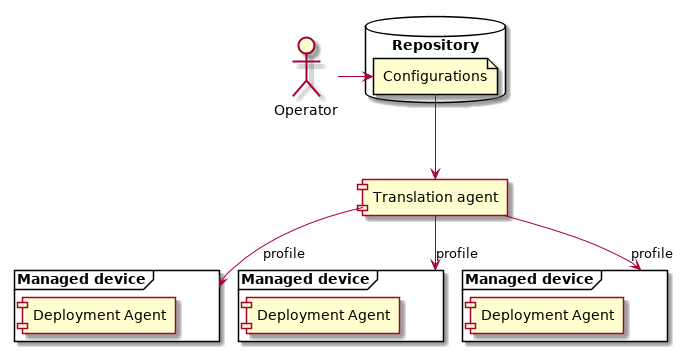
\includegraphics[height=2in]{assets/architecture}
\caption{Architecture of a centralized configuration management tool \cite{delaet2010survey}}
\label{fig:architecture}
\end{figure*}

\subsubsection{Distribution Mechanism}\hfill\\
In order to distribute configurations from the centralized control server there are two mechanisms tools implement.

\begin{description}
	
	\item[Push-based systems] \hfill \\ 
	Configuration is pushed and synchronously applied on the managed hosts. This does not require an agent program to be installed on the machine. 
	
	\item[Pull-based systems] \hfill \\
	Configuration is fetched by the agent program from the centralized control server in regular intervals and changes are applied by the agent program.
	
\end{description}

While Chef and Puppet both are pull-based systems both tools have implemented capabilities to manually trigger configuration distribution outside of the regular pull-schedule.

Pull-based systems have been shown to scale better to a larger number of managed devices.

%WRITTEN BY: Daniel
\subsection{Management}

The configuration management tool does not operate in a vacuum but needs to work well together with existing tools, infrastructure and software development procedures.

\subsubsection{Testing}\hfill\\
Similiar to application code, configuration changes need to be tested before they are applied to the production system. There are a number of different tests that can be used to verify configurations.

\begin{description}
	
	\item[Syntax Checking] \hfill \\ 
	Identification of syntactical mistakes by simulating the interpreter. This is often provided as part of the editing experience inside an editor.
	
	\item[Unit Tests] \hfill \\
	Testing of single functions and units of the configuration to ensure they are behaving as expected.
	
	\item[System / Integration Tests]  \hfill \\
	Testing of multiple configuration components and functions in a simulated environment reflecting the live system.
	
	\item[Dry Runs] \hfill \\
	Configuration Management tools provide facilities to simulate the application of a configuration but does not actually apply it. The simulation is often referred to as a \textit{Dry Run}.	
	
\end{description}


\subsubsection{Monitoring \& Integrations}\hfill\\

Essential for configuration management tools is the integration into the existing tool landscape. Integrations into 

\begin{itemize}
\item Version Control Systems
\item Continous Integration Servers
\item Cloud Platforms
\item Monitoring Systems
\item Access Control Systems
\end{itemize}

are either offered as part of the commercial offering of both tools respectively or contributed by the community.


%WRITTEN BY: Felix
\subsection{Support}

Apart from the technical details, there are further criteria to be considered when selecting a configuration management tool. These criteria concern the ongoing support in terms of maintenance of the tool itself, as well as available technical support when dealing with issues in one's particular setup.

\subsubsection{Documentation}

When getting in touch with a new tool, having sufficient documentation available is key for a steep learning curve. Even when the user is a already familiar with a particular tool, documentation will help by specifying the exact behavior of the tool and describe more efficient ways to achieve a desired goal. This may especially be important, if operations have unintuitive side effects or contain identified bugs.

\todo{Puppet \& Chef}

\subsubsection{Maturity}

When software is just released, there is a high chance for it to crash or behave in an undefined way. Over time, these issues are corrected shortly after detection, so that the software gets more and more stable. When operating critical infrastructure, the maturity of software must therefore be taken into serious consideration to ensure high availability and reliability.

\todo{Puppet \& Chef}

\subsubsection{Commercial support}

The breakdown of critical infrastructure may have a serious impact on its environment. On the other hand, having a sufficiently large team at hand to tackle any issues at all team is extremely costly. Therefore, commercial support plays a critical role in such applications. Commercial support not only allows for quick reaction to failures, but may also offer training opportunities \cite{delaet2010survey}.

\todo{Puppet \& Chef}

\subsubsection{Community}

Apart from the official documentation, there is a lot more information available, mostly created and maintained by the community in the form of forums, wiki's and social networks \cite{delaet2010survey}. Not only do they provide answers to existing questions, but allow active discussions with the community and allow to learn from other users experience. Additionally, the community usually plays an important role in the life-cycle of a tool by creating extensions, reporting bugs or even offering patches. This is especially important if a particular software is open-source and therefore allows direct influence on it's development. GitHub only hosts approximately 85 million projects \cite{githubabout}.

\todo{Puppet \& Chef}
\section{Conclusions}

\begin{itemize}
\item Decision for or against a certain tool might not only be technical but depends on the structure of the organization implementing the architecture (Conways Law?)
\end{itemize}



\bibliographystyle{ACM-Reference-Format}
\bibliography{references}

\end{document}
